\documentclass{article}
\usepackage[margin=1in]{geometry}
\usepackage{tikz}
\usepackage{amsmath}   % <-- Add this for \dfrac
\usepackage{amssymb}   % <-- Add this for \checkmark
\usetikzlibrary{positioning, arrows.meta, shapes.geometric, calc}
\begin{document}

% =============================================================================
% Figure 1: Car Following Analogy (Simple)
% =============================================================================
\begin{figure}[h]
\centering
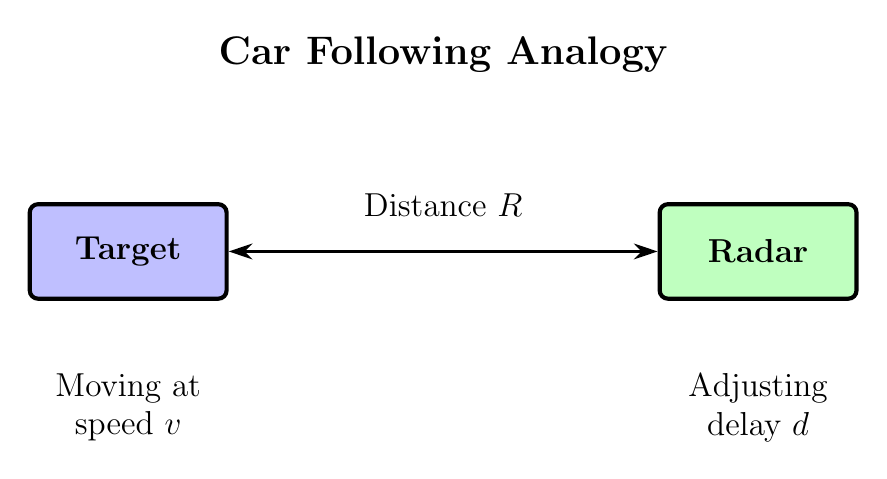
\begin{tikzpicture}[
    car/.style={
        rectangle, 
        draw=black, 
        line width=1.5pt,
        minimum width=2.5cm, 
        minimum height=1.2cm, 
        rounded corners=3pt,
        font=\large\bfseries
    },
    arrow/.style={-{Stealth[length=4mm, width=3mm]}, line width=1.5pt},
    label/.style={font=\large},
    title/.style={font=\Large\bfseries}
]

% Title
\node[title] at (4, 2.5) {Car Following Analogy};

% Target car
\node[car, fill=blue!25] (target) at (0, 0) {Target};
\node[label, below=0.8cm of target, align=center] {Moving at\\speed $v$};

% Radar car
\node[car, fill=green!25] (radar) at (8, 0) {Radar};
\node[label, below=0.8cm of radar, align=center] {Adjusting\\delay $d$};

% Distance arrow (bidirectional)
\draw[{Stealth[length=3mm, width=2mm]}-{Stealth[length=3mm, width=2mm]}, line width=1.2pt] 
    (target.east) -- (radar.west) 
    node[midway, above=0.3cm, font=\large] {Distance $R$};

\end{tikzpicture}
\caption{The radar controller tries to ``follow'' the target by adjusting the delay $d$.}
\end{figure}

% =============================================================================
% Figure 2: Car Following Analogy (Detailed with Wheels)
% =============================================================================
\begin{figure}[h]
\centering
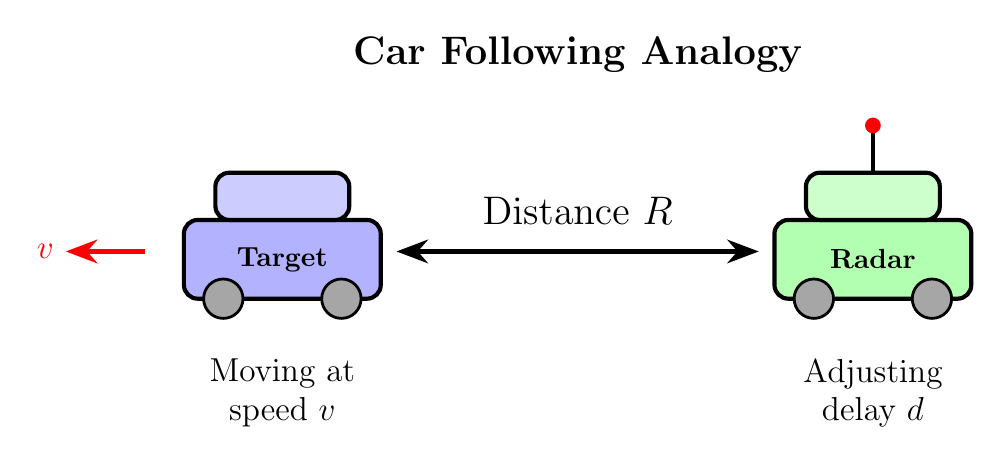
\begin{tikzpicture}[
    wheel/.style={circle, draw=black, fill=gray!70, minimum size=0.5cm, line width=1pt},
    carbody/.style={rectangle, draw=black, line width=1.5pt, rounded corners=5pt},
    label/.style={font=\large},
    title/.style={font=\Large\bfseries}
]

% Title
\node[title] at (5, 3.5) {Car Following Analogy};

% === Target Car ===
\begin{scope}[shift={(0,0)}]
    % Car body
    \draw[carbody, fill=blue!30] (0, 0.4) rectangle (2.5, 1.4);
    % Car top
    \draw[carbody, fill=blue!20] (0.4, 1.4) rectangle (2.1, 2);
    % Wheels
    \node[wheel] at (0.5, 0.4) {};
    \node[wheel] at (2.0, 0.4) {};
    % Label
    \node[font=\bfseries] at (1.25, 0.9) {Target};
\end{scope}

% Target label below
\node[label, align=center] at (1.25, -0.8) {Moving at\\speed $v$};

% Velocity arrow
\draw[-{Stealth[length=4mm, width=3mm]}, line width=2pt, red] 
    (-0.5, 1) -- (-1.5, 1) 
    node[left, font=\large] {$v$};

% === Radar Car ===
\begin{scope}[shift={(7.5,0)}]
    % Car body
    \draw[carbody, fill=green!30] (0, 0.4) rectangle (2.5, 1.4);
    % Car top
    \draw[carbody, fill=green!20] (0.4, 1.4) rectangle (2.1, 2);
    % Wheels
    \node[wheel] at (0.5, 0.4) {};
    \node[wheel] at (2.0, 0.4) {};
    % Label
    \node[font=\bfseries] at (1.25, 0.9) {Radar};
    % Antenna
    \draw[line width=1.5pt] (1.25, 2) -- (1.25, 2.6);
    \fill[red] (1.25, 2.6) circle (0.1);
\end{scope}

% Radar label below
\node[label, align=center] at (8.75, -0.8) {Adjusting\\delay $d$};

% === Distance Arrow ===
\draw[{Stealth[length=4mm, width=3mm]}-{Stealth[length=4mm, width=3mm]}, line width=1.5pt] 
    (2.7, 1) -- (7.3, 1) 
    node[midway, above=0.2cm, font=\Large] {Distance $R$};

\end{tikzpicture}
\caption{Detailed car following analogy with target and radar vehicles.}
\end{figure}

% =============================================================================
% Figure 3: Complete System Diagram
% =============================================================================
\begin{figure}[h]
\centering
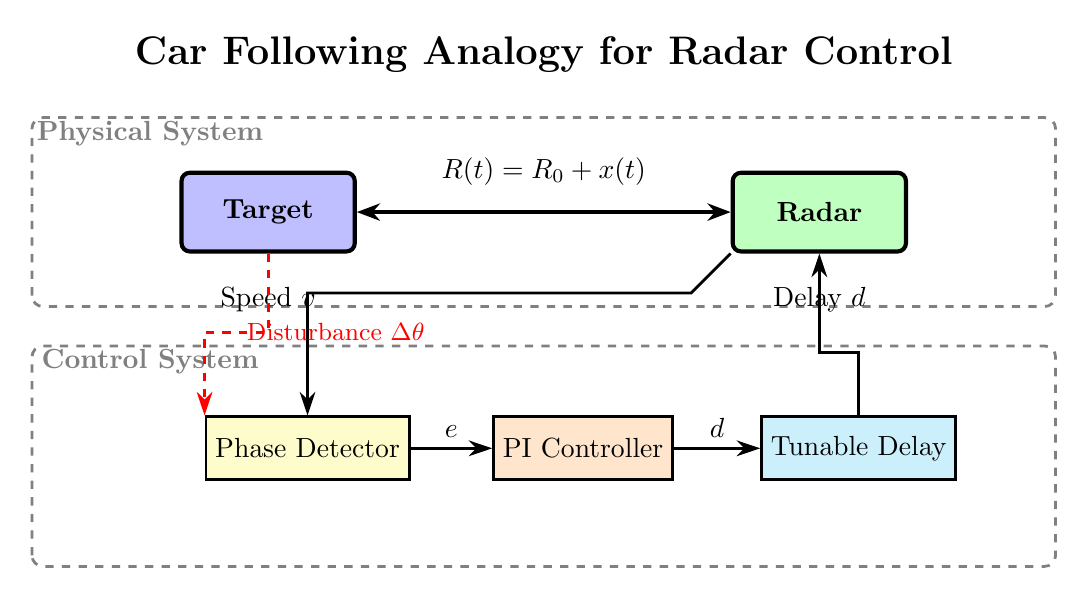
\begin{tikzpicture}[
    car/.style={
        rectangle, 
        draw=black, 
        line width=1.5pt,
        minimum width=2.2cm, 
        minimum height=1cm, 
        rounded corners=3pt,
        font=\normalsize\bfseries
    },
    block/.style={
        rectangle,
        draw=black,
        line width=1pt,
        minimum width=2cm,
        minimum height=0.8cm,
        font=\normalsize
    },
    arrow/.style={-{Stealth[length=3mm, width=2mm]}, line width=1pt},
    label/.style={font=\normalsize},
    title/.style={font=\Large\bfseries}
]

% Title
\node[title] at (5, 5) {Car Following Analogy for Radar Control};

% === Top Section: Physical System ===
\draw[dashed, rounded corners, gray, line width=1pt] (-1.5, 1.8) rectangle (11.5, 4.2);
\node[gray, font=\bfseries] at (0, 4) {Physical System};

% Target car
\node[car, fill=blue!25] (target) at (1.5, 3) {Target};
\node[label, below=0.3cm of target] {Speed $v$};

% Radar car
\node[car, fill=green!25] (radar) at (8.5, 3) {Radar};
\node[label, below=0.3cm of radar] {Delay $d$};

% Distance
\draw[{Stealth}-{Stealth}, line width=1.2pt] (target.east) -- (radar.west)
    node[midway, above=0.2cm] {$R(t) = R_0 + x(t)$};

% === Bottom Section: Control System ===
\draw[dashed, rounded corners, gray, line width=1pt] (-1.5, -1.5) rectangle (11.5, 1.3);
\node[gray, font=\bfseries] at (0, 1.1) {Control System};

% Phase detector
\node[block, fill=yellow!20] (phase) at (2, 0) {Phase Detector};

% Controller
\node[block, fill=orange!20] (ctrl) at (5.5, 0) {PI Controller};

% Delay line
\node[block, fill=cyan!20] (delay) at (9, 0) {Tunable Delay};

% Arrows
\draw[arrow] (phase.east) -- (ctrl.west) node[midway, above] {$e$};
\draw[arrow] (ctrl.east) -- (delay.west) node[midway, above] {$d$};
\draw[arrow] (delay.north) -- ++(0, 0.8) -| (radar.south);
\draw[arrow] (radar.south west) -- ++(-0.5, -0.5) -| (phase.north);

% Disturbance arrow
\draw[arrow, red, dashed] (target.south) -- ++(0, -1) -| (phase.north west)
    node[pos=0.25, right, red, font=\small] {Disturbance $\Delta\theta$};

\end{tikzpicture}
\caption{Complete analogy showing physical system and control system.}
\end{figure}

% =============================================================================
% Figure 4: Speed vs Tracking Capability
% =============================================================================
\begin{figure}[h]
\centering
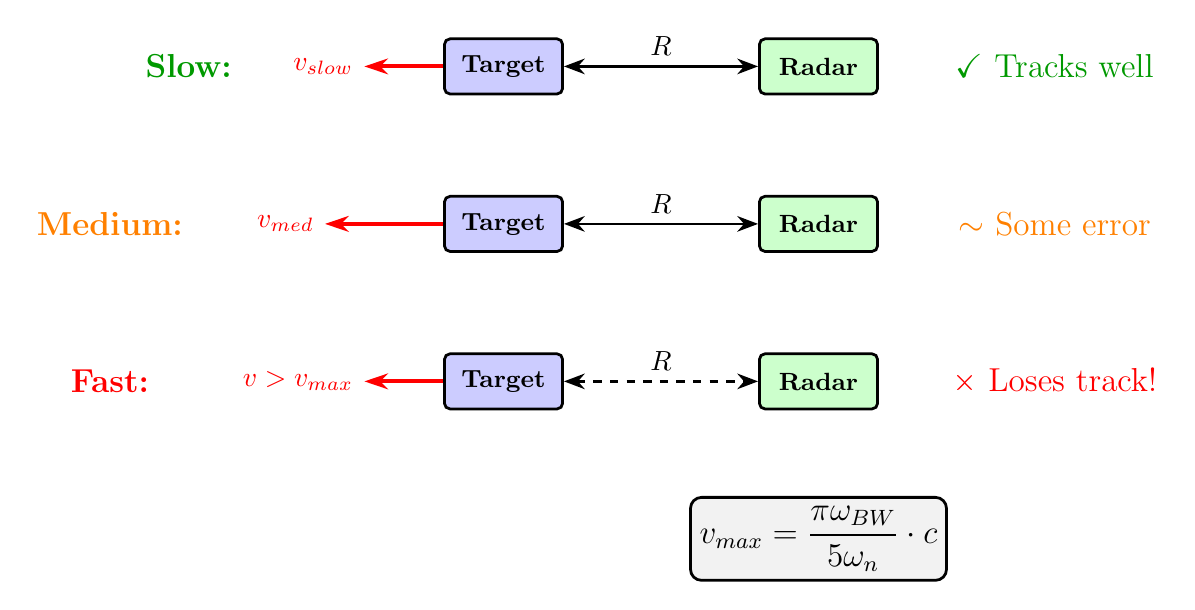
\begin{tikzpicture}[
    car/.style={
        rectangle, 
        draw=black, 
        line width=1pt,
        minimum width=1.5cm, 
        minimum height=0.7cm, 
        rounded corners=2pt,
        font=\small\bfseries
    },
    arrow/.style={-{Stealth[length=3mm, width=2mm]}, line width=1.5pt},
    title/.style={font=\large\bfseries}
]

% === Row 1: Slow Target ===
\node[title, green!60!black] at (-3, 2) {Slow:};
\node[car, fill=blue!20] (t1) at (1, 2) {Target};
\node[car, fill=green!20] (r1) at (5, 2) {Radar};
\draw[{Stealth}-{Stealth}, line width=1pt] (t1.east) -- (r1.west) node[midway, above] {$R$};
\draw[arrow, red] (t1.west) -- ++(-1, 0) node[left] {$v_{slow}$};
\node[green!60!black, font=\large] at (8, 2) {\checkmark\ Tracks well};

% === Row 2: Medium Target ===
\node[title, orange] at (-4, 0) {Medium:};
\node[car, fill=blue!20] (t2) at (1, 0) {Target};
\node[car, fill=green!20] (r2) at (5, 0) {Radar};
\draw[{Stealth}-{Stealth}, line width=1pt] (t2.east) -- (r2.west) node[midway, above] {$R$};
\draw[arrow, red] (t2.west) -- ++(-1.5, 0) node[left] {$v_{med}$};
\node[orange, font=\large] at (8, 0) {$\sim$ Some error};

% === Row 3: Fast Target ===
\node[title, red] at (-4, -2) {Fast:};
\node[car, fill=blue!20] (t3) at (1, -2) {Target};
\node[car, fill=green!20] (r3) at (5, -2) {Radar};
\draw[{Stealth}-{Stealth}, line width=1pt, dashed] (t3.east) -- (r3.west) node[midway, above] {$R$};
\draw[arrow, red] (t3.west) -- ++(-1, 0) node[left] {$v > v_{max}$};
\node[red, font=\large] at (8, -2) {\texttimes\ Loses track!};

% Equation
\node[draw, fill=gray!10, rounded corners, line width=1pt, font=\large] at (5, -4) 
    {$v_{max} = \dfrac{\pi \omega_{BW}}{5\omega_n} \cdot c$};

\end{tikzpicture}
\caption{Effect of target speed on radar tracking capability.}
\end{figure}

\end{document}